% DCGAN 论文简单解读
%   https://www.cnblogs.com/lyrichu/p/9054704.html

% Unsupervised Representation Learning with Deep Convolutional Generative Adversarial Networks
%   https://arxiv.org/abs/1511.06434


\documentclass[a4paper, 12pt]{article}
\usepackage[UTF8]{ctex}
% \usepackage[T1]{fontenc}
% \usepackage{inconsolata}

\usepackage[hidelinks]{hyperref}

\usepackage{amsmath}
\usepackage{enumitem}
\setlist{
    nolistsep, % 去掉 item 和正文之间的间隔
    % labelindent=\parindent,
    leftmargin=*, % 保证小节标签缩进和上面对齐
    % labelsep=1em, % 标签后的空白
    align=left, % 标签对齐段落左边缘
}
\usepackage{tabularx}

\usepackage{graphicx}
\usepackage{subfig}
% \usepackage{subcaption}

\usepackage{geometry}
\geometry{
    a4paper,
    left=2cm,
    right=2cm,
    top=2cm,
    bottom=2cm,
}

\newcommand{\fs}[1]{\fontsize{#1 pt}{0pt}\selectfont}

\usepackage{mathtools}
\DeclarePairedDelimiter{\ceil}{\lceil}{\rceil}
\DeclarePairedDelimiter\floor{\lfloor}{\rfloor}

\usepackage{setspace}
% \setlength\parindent{0pt}
\setlength{\parindent}{2em} % 中文

% \newfontfamily\csl{Consolas}

\usepackage{array}
\newcolumntype{T}{>{\ttfamily}l}
\newcolumntype{Y}{>{\footnotesize\ttfamily}l}
\newcolumntype{y}{>{\footnotesize\ttfamily}c}

\usepackage{longtable}

\newcommand*{\thead}[1]{\multicolumn{1}{c}{\bfseries #1}}
\newcommand*{\yhead}[1]{\multicolumn{1}{c}{\footnotesize\bfseries #1}}

\newcommand{\ssa}{\phantom{x}}
\newcommand{\ssb}{\phantom{xx}}
\newcommand{\ssc}{\phantom{xxx}}
\newcommand{\ssd}{\phantom{xxxx}}
\newcommand{\sse}{\phantom{xxxxx}}

\usepackage{xcolor}
\usepackage{listings}
\definecolor{mygreen}{RGB}{28,172,0} % color values Red, Green, Blue
\definecolor{mylilas}{RGB}{170,55,241}

\newcommand{\ttf}{\ttfamily}

\lstdefinestyle{plainText}{language={},
    basicstyle=\footnotesize \ttfamily,        % set font type and size
    % basicstyle=\ttfamily,        % set font type and size
    breaklines=true,
    keywordstyle=\color{blue},
    % morekeywords={matlab2tikz},
    % morekeywords=[2]{1}, 
    % keywordstyle=[2]{\color{black}},
    identifierstyle=\color{black},
    stringstyle=\color{mylilas},
    % stringstyle=\color{purple},
    frame=single,
    framexleftmargin=0em,
    aboveskip=-\baselineskip,
    commentstyle=\color{mygreen},
    showstringspaces=false,% without this there will be a symbol in the places where there is a space
    % numbers=left,
    numbers=none,
    numberstyle={\tiny \color{black}}, % size of the numbers
    numbersep=9pt, % this defines how far the numbers are from the text
    tabsize=4,                     % sets default tabsize to 4 spaces
    emph=[1]{},
    emphstyle=[1]\color{blue}, %some words to emphasise
    %emph=[2]{word1,word2}, 
    % emphstyle=[2]{style}, 
    escapeinside=``,               % Characters escape: To Use Chinese in codes   
}

\lstdefinestyle{myC}{language={C},
    % basicstyle=\footnotesize \ttfamily,        % set font type and size
    basicstyle=\ttfamily,        % set font type and size
    breaklines=true,
    keywordstyle=\color{blue},
    % morekeywords={matlab2tikz},
    % morekeywords=[2]{1}, 
    % keywordstyle=[2]{\color{black}},
    identifierstyle=\color{black},
    stringstyle=\color{mylilas},
    % stringstyle=\color{purple},
    frame=single,
    framexleftmargin=0em,
    aboveskip=-\baselineskip,
    commentstyle=\color{mygreen},
    showstringspaces=false,% without this there will be a symbol in the places where there is a space
    % numbers=left,
    numbers=none,
    numberstyle={\tiny \color{black}}, % size of the numbers
    numbersep=9pt, % this defines how far the numbers are from the text
    tabsize=4,                     % sets default tabsize to 4 spaces
    emph=[1]{function, return, f, let, add, mult, dot, rk, uw2uwdd, uw2xy1, uw2xy2},
    emphstyle=[1]\color{blue}, %some words to emphasise
    % emph=[2]{word1,word2}, 
    % emphstyle=[2]{style}, 
    escapeinside=``,               % Characters escape: To Use Chinese in codes   
}


\lstdefinestyle{myPython}{language=Python,
    % basicstyle=\footnotesize \ttconsolas,        % set font type and size
    basicstyle=\footnotesize \ttfamily,        % set font type and size
    breaklines=true,
    keywordstyle=\color{blue},
    % morekeywords={matlab2tikz},
    % morekeywords=[2]{1}, 
    % keywordstyle=[2]{\color{black}},
    identifierstyle=\color{black},
    stringstyle=\color{mylilas},
    % stringstyle=\color{purple},
    frame=single,
    framexleftmargin=0em,
    aboveskip=-\baselineskip,
    commentstyle=\color{mygreen},
    showstringspaces=false,% without this there will be a symbol in the places where there is a space
    numbers=left,
    numberstyle={\tiny \color{black}}, % size of the numbers
    numbersep=9pt, % this defines how far the numbers are from the text
    tabsize=4,                     % sets default tabsize to 4 spaces
    emph=[1]{nonLinearFunction, bitReorganization, modAdd_2e31m1, binaryAdd, binaryXor, sboxOfZuc, linearTransform},
    emphstyle=[1]\color{red}, %some words to emphasise
    %emph=[2]{word1,word2}, 
    % emphstyle=[2]{style}, 
    escapeinside=``,               % Characters escape: To Use Chinese in codes   
}


\begin{document}


\includepdf[]{./images/cover.pdf}

\setcounter{page}{1}

\begin{center}
{\fs{20}\textbf{基于 MNIST 数据集使用 CGAN 生成手写数字}}

\vspace{2\baselineskip}
{\fs{16}于泽汉 \hspace{1.5ex} 118039910141}

\vspace{1.5\baselineskip}

{\fs{16}yuzehan002@126.com}

\vspace{2\baselineskip}

{\fs{16}\textbf{摘要}}

\end{center}

本文基于 MNIST 数据集,采用 TensorFlow 框架,实现了条件生成对抗网络(CGAN) 模型,生成了指定的手写数字。

经典的 GAN 是非监督式学习的一种方法,通过让两个神经网络相互博弈的方式进行学习,其主要组成部分是一个生成网络(G)与一个判别网络(D)。

而 CGAN 则对 GAN 作了改进,在生成模型(G)和判别模型(D)的建模中均引入条件变量 y,使用额外信息y对模型增加条件,可以指导数据生成过程。

另一种对 GAN 的改进模型是 DCGAN(深度卷积生成对抗网络),本文也对其作了简要的说明。

实验结果表明,CGAN 在生成手写数字方面表现很好,并且弥补了 GAN 不能指定生成数据类别的缺点。同时,CGAN 比 DCGAN 的学习速度更快,而学习效果并没有明显区别。

\vspace{\baselineskip}

\textbf{关键词:} CGAN,MNIST,神经网络,机器学习,图像处理

\newpage

% 题目、摘要、问题描述、模型建立与求解过程、代码实现、结果与分析、参考文献
% 期末报告基本要求:(1)模型建立和理论求解过程。例如,数据的处理方式?求解方法的选择?参数的控制和调节? (2)代码实现过程:原始代码+代码注释+结果展示,需说明运行平台。

\section{问题描述}
在 Windows 10 操作系统上,基于 MNIST 数据集,采用 Python + TensorFlow 平台,实现条件生成对抗网络(CGAN) 模型,生成指定的手写数字。

报告要求:
\begin{enumerate}[leftmargin=*,labelindent=2em]
\item 模型建立和理论求解过程。例如,数据的处理方式?求解方法的选择?参数的控制和调节?方法讨论等。
\item 代码实现过程:原始代码+代码注释+结果展示。
\item 报告需要包含:题目、摘要、问题描述、模型建立与求解过程、代码实现、结果与分析、参考文献。
\end{enumerate}

\section{模型建立与求解}
\subsection{生成对抗网络(GAN)}

生成对抗网络(Generative Adversarial Network,简称GAN)是非监督式学习的一种方法,通过让两个神经网络相互博弈的方式进行学习。该方法由伊恩·古德费洛等人于2014年提出。

生成对抗网络由一个生成网络与一个判别网络组成。

生成网络从潜在空间中随机取样作为输入,其输出结果需要尽量模仿训练集中的真实样本。判别网络的输入则为真实样本或生成网络的输出,其目的是将生成网络的输出从真实样本中尽可能分辨出来。而生成网络则要尽可能地欺骗判别网络。两个网络相互对抗、不断调整参数,最终目的是使判别网络无法判断生成网络的输出结果是否真实。

生成对抗网络常用于生成以假乱真的图片。此外,该方法还被用于生成影片、三维物体模型等。

虽然生成对抗网络原先是为了无监督学习提出的,它也被证明对半监督学习、完全监督学习、强化学习是有用的。Yann Le Cun 曾评价道,生成式对抗网络是“机器学习这二十年来最酷的想法”。

\begin{figure}[htbp]
\centering
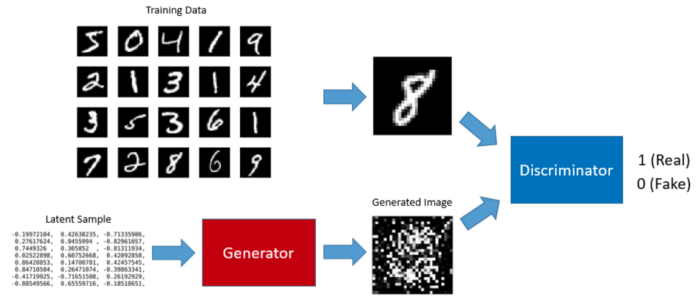
\includegraphics[width=0.8\textwidth]{images/gan_structure.png}
\caption{GAN 生成手写数字的流程}
\end{figure}


\subsection{条件生成对抗网络(CGAN)}

与其他生成式模型相比,GAN 这种竞争的方式不再要求一个假设的数据分布,而是使用一种分布直接进行采样,从而真正达到理论上可以完全逼近真实数据,这也是GAN最大的优势。

然而,这种不需要预先建模的方法缺点是太过自由了,对于较大的图片,使用经典 GAN 时可控性明显下降。

为了解决 GAN 太过自由这个问题,一个很自然的想法是给 GAN 加一些约束,于是便有了条件生成对抗网络(Conditional Generative Adversarial Nets,简称 CGAN)。

这项工作提出了一种带条件约束的 GAN,在生成模型(G)和判别模型(D)的建模中均引入条件变量 y,使用额外信息 y 对模型增加条件,可以指导数据生成过程。

这些条件变量 y 可以基于多种信息,例如类别标签、用于图像修复的部分数据或者说来自不同模态的数据。如果条件变量 y 是类别标签,可以认为 CGAN 是把纯无监督的 GAN 改进为有监督的 GAN。

实践证明,这个简单直接的改进非常有效,并广泛用于后续的相关工作中。

Mehdi Mirza 等人的工作是在 MNIST 数据集上以类别标签为条件变量,生成指定类别的图像。作者还探索了 CGAN 在用于图像自动标注的多模态学习上的应用,在 MIR Flickr25000 数据集上,以图像特征为条件变量,生成该图像的标签的词向量。

\begin{figure}[htbp]
\centering
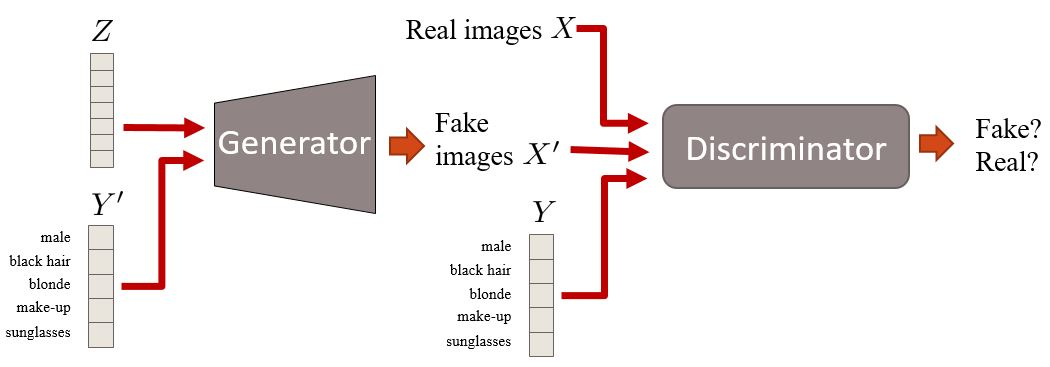
\includegraphics[width=\textwidth]{images/cgan_structure.jpg}
\caption{CGAN 只是在 GAN 的基础上增加了条件变量}
\end{figure}

\subsection{MNIST 数据集}
MNIST 数据集(Modified National Institute of Standards and Technology database)是一个手写数字的大型数据库,通常用于训练各种图像处理系统。

该数据库广泛用于机器学习领域的训练和测试。它是通过“重新混合”来自 NIST 原始数据集的样本而创建的。MNIST 数据集的创建者认为,由于 NIST 的训练数据集是从美国人口普查局的雇员那里获取的,而测试数据集却来自美国高中生,因此它不太适合机器学习实验。此外,MNIST 还将 NIST 原始数据集 的黑白图像标准化,以匹配 $28 \times 28$ 像素边界框,并且引入了灰度级别,以消除锯齿。

MNIST 数据集包含了 60000 个训练图像和 10000 个测试图像。


\begin{figure}[htbp]
\centering
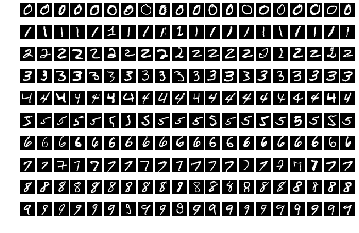
\includegraphics[width=0.8\textwidth]{images/dataset_preview.png}
\caption{MNIST 数据集中手写数字 0 - 9 的图像}
\end{figure}

\section{代码实现与说明}

\subsection{创建生成器和判别器}
这里使用带泄露的线性整流函数,而不是经典的线性整流函数,目的是避免某些神经元过早“死亡”(对任何输入都输出 0),也就是所谓的“Dead ReLU”问题。

\begin{lstlisting}[style=myPython,caption={带泄露的线性整流函数}]
def leakyRELU(X, leak=0.2):
    f1 = 0.5 * (1 + leak)
    f2 = 0.5 * (1 - leak)
    return f1 * X + f2 * tf.abs(X)
\end{lstlisting}

本文使用的生成器 G 结构如下:

\begin{enumerate}[leftmargin=*,labelindent=2em]
\item 输入层:$110$ 个节点 = ($100 \times 1$ 的随机噪声 $z$) + ($10 \times 1$ 的条件变量 $y$)
\item 隐藏层:$128$ 个节点的全连接层,激活函数为 ReLU
\item 输出层:$784$ 个节点的全连接层,激活函数为 tanh
\end{enumerate}

\begin{lstlisting}[style=myPython,caption={生成器 G}]
def generator(x, y, isTrain=True, reuse=False):
    with tf.variable_scope('generator', reuse=reuse):
        w_init = tf.contrib.layers.xavier_initializer()
        cat1 = tf.concat([x, y], 1)
        dense1 = tf.layers.dense(cat1, 128, kernel_initializer=w_init)
        relu1 = tf.nn.relu(dense1)
        dense2 = tf.layers.dense(relu1, 784, kernel_initializer=w_init)
        out = tf.nn.tanh(dense2)
        return out
\end{lstlisting}

本文使用的判别器 D 结构如下:
\begin{enumerate}[leftmargin=*,labelindent=2em]
\item 输入层:$110$ 个节点 = ($100 \times 1$ 的随机噪声 $z$) + ($10 \times 1$ 的条件变量 $y$)
\item 隐藏层:$128$ 个节点的全连接层,激活函数为 ReLU
\item 输出层:$1$ 个节点的全连接层,激活函数为 sigmoid
\end{enumerate}

\begin{lstlisting}[style=myPython,caption={判别器 D}]
def discriminator(x, y, isTrain=True, reuse=False):
    with tf.variable_scope('discriminator', reuse=reuse):
        w_init = tf.contrib.layers.xavier_initializer()
        cat1 = tf.concat([x, y], 1)
        dense1 = tf.layers.dense(cat1, 128, kernel_initializer=w_init)
        relu1 = leakyRELU(dense1, 0.2)
        dense2 = tf.layers.dense(relu1, 1, kernel_initializer=w_init)
        out = tf.nn.sigmoid(dense2)
        return out, dense2
\end{lstlisting}

\subsection{初始化随机噪声和条件变量(图像类别)}

生成的图像共有 $10 \times 10 = 100$ 个,其中每一行代表同一个数字。

每个随机噪声在生成后就不再改变,这些随机噪声用作生成器的输入。

每一行数字使用同一个条件变量,代表图像类别,采用独热码(one hot)的形式。

\begin{lstlisting}[style=myPython,caption={初始化随机噪声和条件变量(图像类别)}]
onehot = np.eye(10)
temp_z_ = np.random.normal(0, 1, (10, 100))
fixed_z_ = temp_z_
fixed_y_ = np.zeros((10, 1))
for i in range(9):
    fixed_z_ = np.concatenate([fixed_z_, temp_z_], 0)
    temp = np.ones((10,1)) + i
    fixed_y_ = np.concatenate([fixed_y_, temp], 0)
fixed_y_ = onehot[fixed_y_.astype(np.int32)].squeeze()
\end{lstlisting}

\subsection{记录中间结果和相关信息}

这个函数用于将每个 Epoch 训练中生成的图像保存下来,以备后续的分析。

\begin{lstlisting}[style=myPython,caption={记录中间结果和相关信息}]
def recordResult(num_epoch, show=False, save=False, path='result.png'):
    test_images = sess.run(G_z, {z: fixed_z_, y: fixed_y_, isTrain: False})
    size_figure_grid = 10
    fig,ax = plt.subplots(size_figure_grid,size_figure_grid,figsize=(5,5))
    for i,j in itertools.product(range(size_figure_grid), range(size_figure_grid)):
        ax[i,j].get_xaxis().set_visible(False)
        ax[i,j].get_yaxis().set_visible(False)
    for k in range(size_figure_grid*size_figure_grid):
        i = k // size_figure_grid
        j = k % size_figure_grid
        ax[i,j].cla()
        ax[i,j].imshow(np.reshape(test_images[k], (28, 28)), cmap='gray')
    label = 'Epoch {0}'.format(num_epoch)
    fig.text(0.5, 0.04, label, ha='center')
    if save:
        plt.savefig(path)
    if show:
        plt.show()
    else:
        plt.close()
\end{lstlisting}

\subsection{绘制损失函数曲线}

这个函数用于绘制生成器和判别器的损失函数曲线,将其损失的变化可视化出来。

\begin{lstlisting}[style=myPython,caption={绘制损失函数曲线}]
def plotLoss(hist, show = False, save = False, path = 'Train_hist.png'):
    x = range(len(hist['D_losses']))
    y1 = hist['D_losses']
    y2 = hist['G_losses']
    plt.plot(x, y1, label='D_loss')
    plt.plot(x, y2, label='G_loss')
    plt.xlabel('Epoch')
    plt.ylabel('Loss')
    plt.legend(loc=1)
    plt.grid(True)
    plt.tight_layout()
    if save:
        plt.savefig(path)
    if show:
        plt.show()
    else:
        plt.close()
\end{lstlisting}

\subsection{训练过程}

\subsubsection{设置超参数}

设置训练中使用的超参数,包括批处理大小(BATCH\_SIZE)、学习率(LEARNING\_RATE)和迭代全训练集的次数(EPOCHS)等。

这里的超参数需要根据数据集本身的特点和训练结果,不断调整,以达到最优的效果。

批处理大小越大,训练速度越快,越能提取数据集总体特征,但是单个 Epoch 迭代的次数也越少,收敛得也越慢。这里选用的值为 150。

学习率越高,收敛速度越快,但是学习率过大,会导致越过最优值,产生振荡,而学习率过小,则会严重影响优化的效率。这里选用的值为 0.001。

迭代全训练集的次数越多,越能接近学习效果的上限,当然,耗费的时间也越久。到一定次数后,学习效果将不再提升。这里选用的值为 200。

\begin{lstlisting}[style=myPython,caption={设置超参数}]
BATCH_SIZE = 150
LEARNING_RATE = 0.001
EPOCHS = 200
\end{lstlisting}

\subsubsection{导入 MNIST 数据集}

导入 MNIST 数据集,并且作相应的预处理,以用于之后的训练。

\begin{lstlisting}[style=myPython,caption={导入 MNIST 数据集}]
mnist = input_data.read_data_sets("MNIST_data/", one_hot=True)
train_set = (mnist.train.images - 0.5) / 0.5  # normalization; range: -1 ~ 1
train_label = mnist.train.labels
\end{lstlisting}

\subsubsection{创建相关的变量,和中间变量保存的列表}

\begin{lstlisting}[style=myPython,caption={创建输入变量 $x$、随机噪声 $z$、条件变量 $y$}]
`\cmt{\# x: 输入变量}`
x = tf.placeholder(tf.float32, shape=(None, 784))
`\cmt{\# y: 条件变量(图像类别)}`
y = tf.placeholder(tf.float32, shape=(None, 10))
`\cmt{\# z: 随机噪声}`
z = tf.placeholder(tf.float32, shape=(None, 100))
\end{lstlisting}

\begin{lstlisting}[style=myPython,caption={设置结果保存路径,创建中间变量保存数组}]
`\cmt{\# 设置结果保存路径}`
root = 'MNIST_cGAN_results/'
model = 'MNIST_cGAN_'
if not os.path.isdir(root):
    os.mkdir(root)
if not os.path.isdir(root + 'Fixed_results'):
    os.mkdir(root + 'Fixed_results')
`\cmt{\# 创建中间变量保存数组}`
train_hist = {}
train_hist['D_losses'] = []
train_hist['G_losses'] = []
train_hist['per_epoch_ptimes'] = []
train_hist['total_ptime'] = []
\end{lstlisting}

\subsubsection{实例化生成器和判别器}

需要注意的是,判别器包含两部分,即对真图像的判别,和对假图像的判别。

\begin{lstlisting}[style=myPython,caption={实例化生成器和判别器}]
`\cmt{\# 实例化生成器}`
G_z = generator(z, y, isTrain)
`\cmt{\# 实例化判别器}`
D_real, D_real_logits = discriminator(x, y, isTrain)
D_fake, D_fake_logits = discriminator(G_z, y, isTrain, reuse=True)
\end{lstlisting}

\subsubsection{设置损失值变量、每层网络的可训练变量以及优化器}

这一步涉及到对网络的优化。

需要注意的是,判别器的损失函数包括两部分,即其值应为相对真图像的损失和假图像的损失之和。

本文采用 Adam 优化器,能够控制学习速度,经过偏置校正后,每一次迭代学习率都有个确定范围,使参数变化较为平稳。

\begin{lstlisting}[style=myPython,caption={设置损失值变量、每层网络的可训练变量以及优化器}]
`\cmt{\# 设置损失值变量}`
D_loss_real = tf.reduce_mean(tf.nn.sigmoid_cross_entropy_with_logits(logits=D_real_logits, labels=tf.ones([BATCH_SIZE, 1])))
D_loss_fake = tf.reduce_mean(tf.nn.sigmoid_cross_entropy_with_logits(logits=D_fake_logits, labels=tf.zeros([BATCH_SIZE, 1])))
D_loss = D_loss_real + D_loss_fake
G_loss = tf.reduce_mean(tf.nn.sigmoid_cross_entropy_with_logits(logits=D_fake_logits, labels=tf.ones([BATCH_SIZE, 1])))

`\cmt{\# 设置每层网络的可训练变量}`
T_vars = tf.trainable_variables()
D_vars = [var for var in T_vars if var.name.startswith('discriminator')]
G_vars = [var for var in T_vars if var.name.startswith('generator')]

`\cmt{\# 设置每层网络的的优化器}`
with tf.control_dependencies(tf.get_collection(tf.GraphKeys.UPDATE_OPS)):
    D_optim = tf.train.AdamOptimizer(LEARNING_RATE, beta1=0.5).minimize(D_loss, var_list=D_vars)
    G_optim = tf.train.AdamOptimizer(LEARNING_RATE, beta1=0.5).minimize(G_loss, var_list=G_vars)
\end{lstlisting}

\subsubsection{开始训练}

这部分对数据集进行训练,记录并输出中间结果,并保存训练得到的模型。

\begin{lstlisting}[style=myPython,caption={启动 TensorFlow 会话,初始化所有变量}]
sess = tf.InteractiveSession()
tf.global_variables_initializer().run()
\end{lstlisting}

\begin{lstlisting}[style=myPython,caption={对数据集进行训练,并输出中间结果}]
np.random.seed(int(time.time()))
print('+ Training start!')
start_time = time.time()
for epoch in range(EPOCHS):
    G_losses = []
    D_losses = []
    epoch_start_time = time.time()
    for iter in range(len(train_set) // BATCH_SIZE):
        `\cmt{\# 更新判别器}`
        x_ = train_set[iter * BATCH_SIZE:(iter + 1) * BATCH_SIZE]
        y_ = train_label[iter * BATCH_SIZE:(iter + 1) * BATCH_SIZE]
        z_ = np.random.normal(0, 1, (BATCH_SIZE, 100))
        loss_d_, _ = sess.run([D_loss, D_optim], {x: x_, y: y_, z: z_, isTrain: True})
        D_losses.append(loss_d_)
        `\cmt{\# 更新生成器}`
        z_ = np.random.normal(0, 1, (BATCH_SIZE, 100))
        y_ = np.random.randint(0, 10, (BATCH_SIZE, 1))
        y_ = onehot[y_.astype(np.int32)].squeeze()
        loss_g_, _ = sess.run([G_loss, G_optim], {z: z_, x: x_, y: y_, isTrain: True})
        G_losses.append(loss_g_)
    `\cmt{\# 记录并输出中间结果}`
    epoch_end_time = time.time()
    per_epoch_ptime = epoch_end_time - epoch_start_time
    print('[%3d/%d] ptime: %.2f | d_loss: %.3f | g_loss: %.3f' % ((epoch + 1), EPOCHS, per_epoch_ptime, np.mean(D_losses), np.mean(G_losses)))
    fixed_p = root + 'Fixed_results/' + model + str(epoch + 1) + '.png'
    recordResult((epoch + 1), save=True, path=fixed_p)
    train_hist['D_losses'].append(np.mean(D_losses))
    train_hist['G_losses'].append(np.mean(G_losses))
    train_hist['per_epoch_ptimes'].append(per_epoch_ptime)

`\cmt{\# 输出最终结果}`
end_time = time.time()
total_ptime = end_time - start_time
train_hist['total_ptime'].append(total_ptime)
print('= Avg ptime per epoch: %.3f | total %d epochs time: %.3f' % (np.mean(train_hist['per_epoch_ptimes']), EPOCHS, total_ptime))
print("+ Training finished! Saving training results ...")

`\cmt{\# 保存训练得到的模型}`
with open(root + model + 'train_hist.pkl', 'wb') as f:
    pickle.dump(train_hist, f)

`\cmt{\# 绘制损失函数曲线}`
plotLoss(train_hist, save=True, path=root + model + 'train_hist.png')
\end{lstlisting}


\section{结果与分析}

\subsection{使用 CGAN 生成的手写数字图像效果随训练的 epoch 数变化情况}

在经过不同 Epoch 训练后,生成的手写数字如图 \ref{fig:cgan_imgs} 所示。

从图中可以看出:

\begin{enumerate}[leftmargin=*,labelindent=2em]

\item 在前 20 个 Epoch,生成的手写数字图像还是非常粗糙,几乎不能分辨属于哪个数字。

\item 从第 20 个 Epoch 开始,已经有了模糊的轮廓,不同行的数字也有了一定的区别。尤其是对于 0 和 1 这类特征较为明显的数字,网络已经能比较好地将其生成出来。

\item 之后随着 Epoch 数的增加,生成的不同数字彼此之间差别渐渐变大,图像的轮廓也渐渐清晰。

\item 从第 75 个 Epoch 开始,生成的图像基本稳定,不再发生大的变化。这表明网络已经基本收敛。这一点从后文的损失函数曲线也能够印证。

\item 从最终生成的结果来看,我们的网络训练得还是很好的,基本上学习到了每一类数字的主要特征。

\item 值得注意的是,不同的初始随机数种子,会对生成的图像产生较大的影响。
比如在 Epoch 200 时,生成的图像中的第 3 列和第 9 列,不同数字之间的差别就很小,图像自身的轮廓也较为模糊。其他列的生成效果就相对较好。

\item 这说明我们的生成器还没有足够稳定,对于某些输入的随机量还不能很好地生成对应的手写数字图像。
这是 GAN 固有的缺点,从实验结果确实可见一斑。
\end{enumerate}


\begin{figure}[htbp]
    \centering
    \subfloat[Epoch 1]{%
        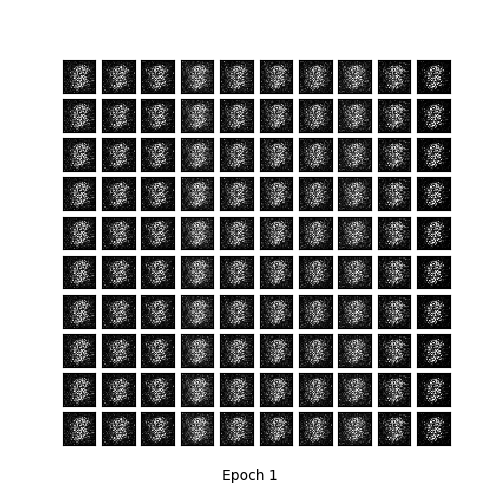
\includegraphics[width=0.45\textwidth]{./images/MNIST_cGAN_1.png}}
    % \phantom{123}
    \subfloat[Epoch 10]{%
        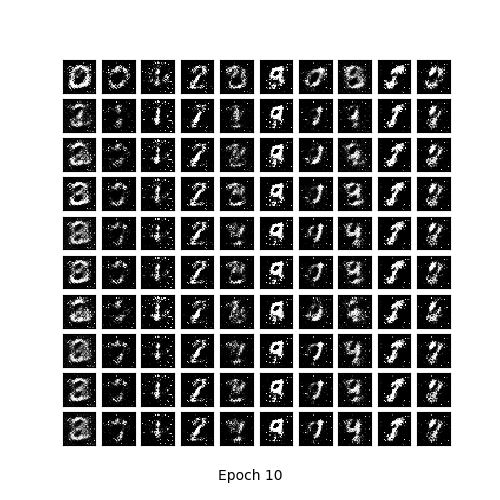
\includegraphics[width=0.45\textwidth]{./images/MNIST_cGAN_10.png}}\\

    % \phantom{123}
    \subfloat[Epoch 20]{%
        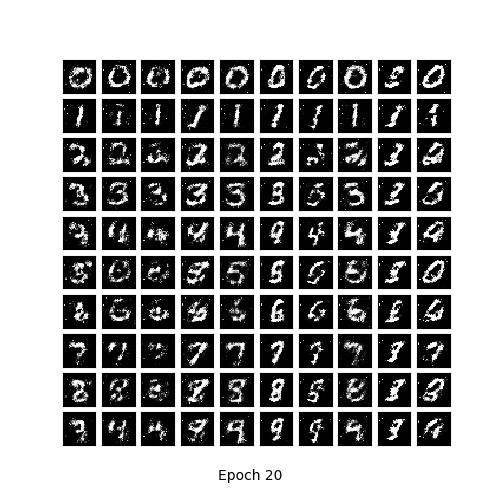
\includegraphics[width=0.45\textwidth]{./images/MNIST_cGAN_20.png}}
    % \phantom{123}
    \subfloat[Epoch 50]{%
        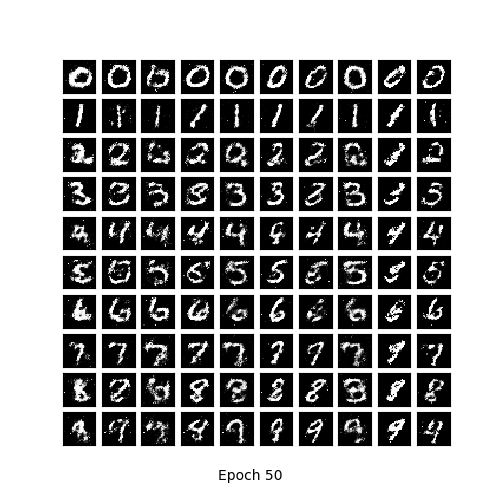
\includegraphics[width=0.45\textwidth]{./images/MNIST_cGAN_50.png}}\\
    \caption{生成的手写数字图像效果随训练的 Epoch 数变化情况}
    \label{fig:cgan_imgs}
\end{figure}

\begin{figure}[htbp]
\ContinuedFloat
\centering
    % \phantom{123}
    \subfloat[Epoch 75]{%
        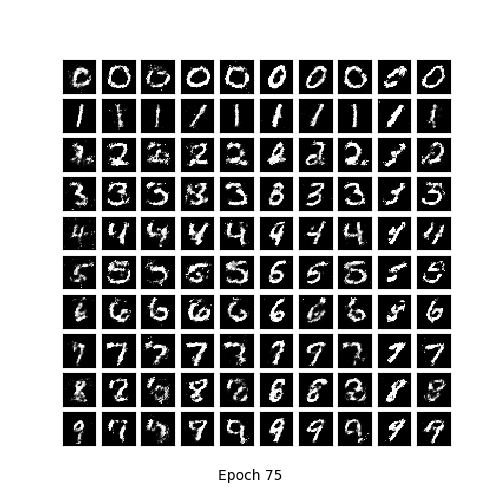
\includegraphics[width=0.45\textwidth]{./images/MNIST_cGAN_75.png}}
    % \phantom{123}
    \subfloat[Epoch 100]{%
        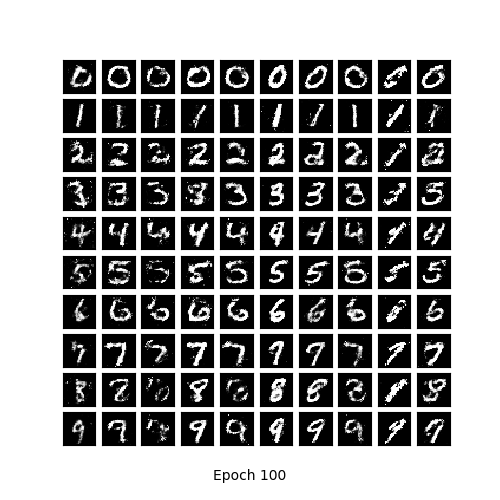
\includegraphics[width=0.45\textwidth]{./images/MNIST_cGAN_100.png}}\\
    % \phantom{123}
    \subfloat[Epoch 150]{%
        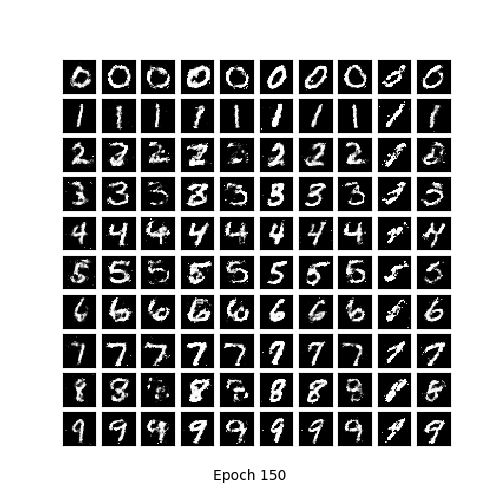
\includegraphics[width=0.45\textwidth]{./images/MNIST_cGAN_150.png}}
    % \phantom{123}
    \subfloat[Epoch 200]{%
        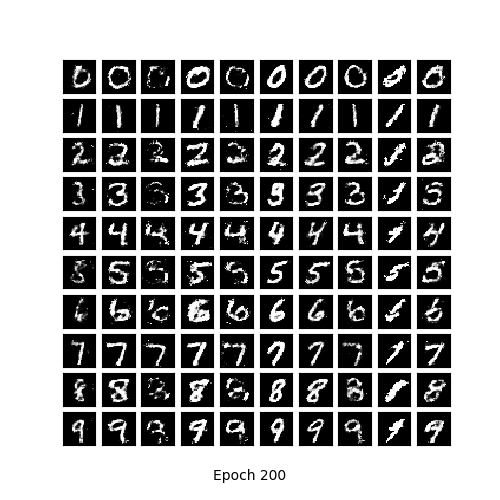
\includegraphics[width=0.45\textwidth]{./images/MNIST_cGAN_200.png}}\\

    \label{fig:cgan_imgs_x}
    \caption{生成的手写数字图像效果随训练的 Epoch 数变化情况(续)}
\end{figure}


\subsection{生成器和判别器的损失函数值随训练的 Epoch 数变化情况}
生成器和判别器的损失函数值随训练的 Epoch 数变化情况如图 \ref{fig:loss} 所示。

从图中可以看出:

\begin{enumerate}[leftmargin=*,labelindent=2em]
\item 生成器 G 的损失值开始较大,之后逐渐减小,直到趋于稳定。
\item 判别器 D 的损失值开始较小,之后逐渐增大,直到趋于稳定
\item 从第 60 个 Epoch 开始,生成器和判别器的损失值都趋于稳定。这一点投我们上面给出的生成图像效果是一致的。
\item 在刚开始训练时,二者的损失值会出现较大的波动。
\item 到训练后期,二者的损失值都有较小的背离理想趋势的变化,这表明已经有轻微的过拟合。

\end{enumerate}

\begin{figure}[htbp]
\centering
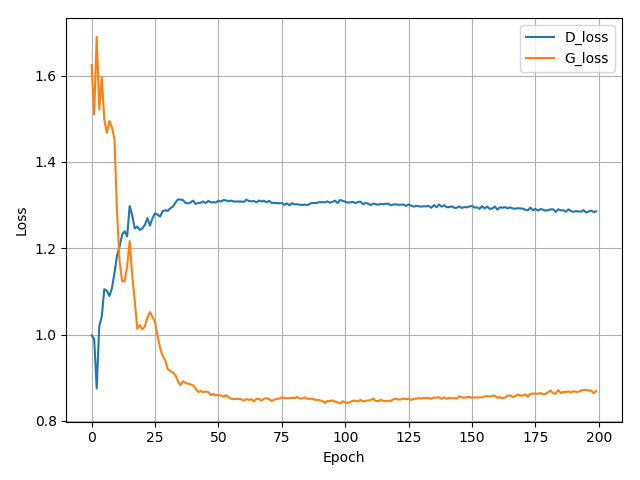
\includegraphics[width=\textwidth]{./images/MNIST_cGAN_loss.png}
\caption{生成器和判别器的损失函数值随训练的 Epoch 数变化情况}
\label{fig:loss}
\end{figure}

\newpage

\subsection{训练耗时}

每个 Epoch 的训练耗时如 Listing \ref{lst:ptime} 所示。

\begin{lstlisting}[style=myPlain,caption={每个 Epoch 的训练耗时},label={lst:ptime}]
[  1/200] ptime: 1.63 | d_loss: 0.998 | g_loss: 1.624
[  2/200] ptime: 1.45 | d_loss: 0.990 | g_loss: 1.510
[  3/200] ptime: 1.44 | d_loss: 0.875 | g_loss: 1.690
...
[ 51/200] ptime: 1.39 | d_loss: 1.310 | g_loss: 0.860
[ 52/200] ptime: 1.50 | d_loss: 1.308 | g_loss: 0.859
...
[100/200] ptime: 1.38 | d_loss: 1.310 | g_loss: 0.846
[101/200] ptime: 1.47 | d_loss: 1.308 | g_loss: 0.842
...
[198/200] ptime: 1.36 | d_loss: 1.287 | g_loss: 0.870
[199/200] ptime: 1.37 | d_loss: 1.284 | g_loss: 0.864
[200/200] ptime: 1.37 | d_loss: 1.285 | g_loss: 0.869
\end{lstlisting}

\vspace{0.5\baselineskip}

单个 Epoch 的平均训练时长与总的训练时长如 Listing \ref{lst:ttime} 所示。

从中可以看出:

\begin{enumerate}[leftmargin=*,labelindent=2em]
\item 我们实现的 CGAN 平均每个 Epoch 耗时约 1.5 秒,速度还是非常快的。
\item 200 个 Epoch 总耗时 743 秒,可见有近一半时间花费在训练之外的处理上了。
\item 在使用 CDCGAN 训练时,平均每个 Epoch 耗时将近 80 秒,速度远慢于 CGAN。
\end{enumerate}

\begin{lstlisting}[style=myPlain,caption={单个 Epoch 的平均训练时长与总的训练时长},label={lst:ttime}]
Average ptime per epoch: 1.472
Total 200 epochs time: 743.067
\end{lstlisting}

\subsection{原始图像、CGAN 生成和 CDCGAN 生成的手写数字图像效果对比}
原始图像、CGAN 生成和 CDCGAN 生成的手写数字图像效果对比如图 \ref{fig:comp} 所示。

从图中可以看出:

\begin{enumerate}[leftmargin=*, labelindent=2em]
\item CGAN 和 CDCGAN 基本上都能生成特征较为明显的手写数字图像,表明 GAN 在这项工作上表现非常出色。
\item 要达到相同的效果,CDCGAN 所需的 Epoch 数明显较少,尽管每个 Epoch 的时间要长很多。
\item CDCGAN 能达到的生成效果的上限,要高于 CGAN,尽管 CGAN 生成的图像效果也已经足够好了。
\end{enumerate}

\begin{figure}[htbp]
    \centering
    \subfloat[原始图像]{%
        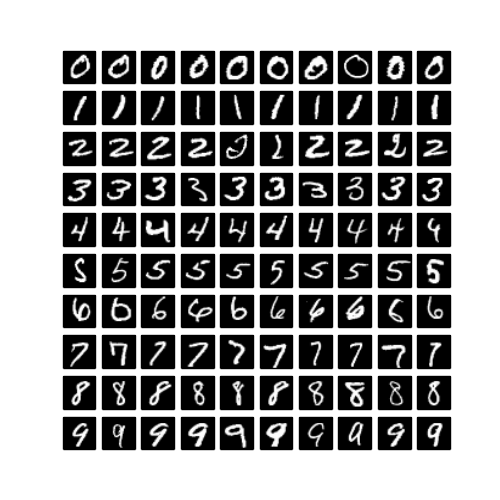
\includegraphics[width=0.35\textwidth]{./images/MNIST_raw.png}}
    % \phantom{123}
    \subfloat[CGAN: Epoch 100]{%
        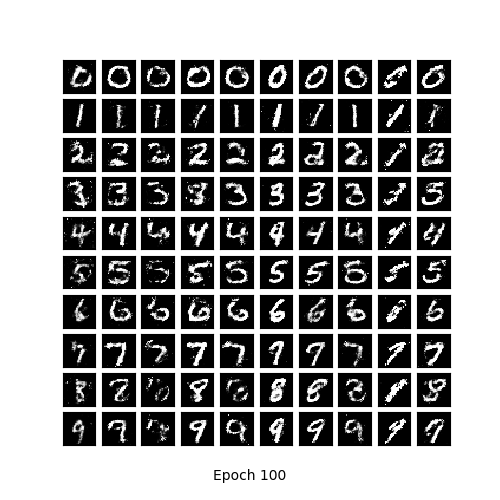
\includegraphics[width=0.35\textwidth]{./images/MNIST_cGAN_100.png}}
    % \phantom{123}
    \subfloat[CDCGAN: Epoch 30]{%
        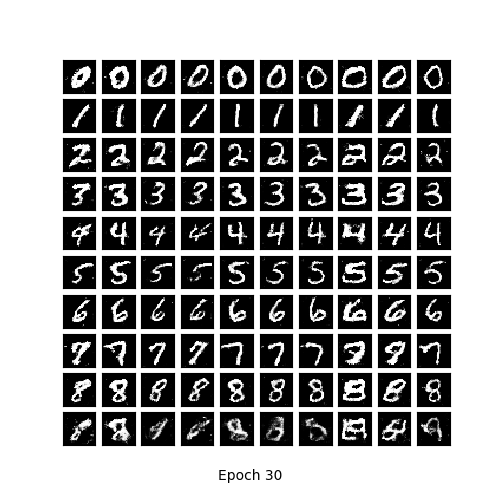
\includegraphics[width=0.35\textwidth]{./images/MNIST_cDCGAN_30.png}}
    \caption{原始图像、CGAN 生成和 CDCGAN 生成的手写数字图像效果对比}
    \label{fig:comp}
\end{figure}

\section{参考文献}

\begin{enumerate}
\item Wikipedia contributors. (2019, July 10). Generative adversarial network. In Wikipedia, The Free Encyclopedia. Retrieved 14:58, July 14, 2019, from \url{https://en.wikipedia.org/w/index.php?title=Generative_adversarial_network&oldid=905621379}

\item Ian J. Goodfellow, Jean Pouget-Abadie, Mehdi Mirza, Bing Xu, David Warde-Farley, Sherjil Ozair, Aaron Courville, Yoshua Bengio. Generative Adversarial Networks. arXiv:1406.2661 [stat.ML]. (Submitted on 10 Jun 2014) \url{https://arxiv.org/abs/1406.2661}

\item LeCun, Y. \& Cortes, C. (2010). MNIST handwritten digit database. , .  \url{http://yann.lecun.com/exdb/mnist/}

\item Mehdi Mirza, Simon Osindero. Conditional Generative Adversarial Nets. arXiv:1411.1784 [cs.LG]. (Submitted on 6 Nov 2014) \url{https://arxiv.org/abs/1411.1784}

\item Alec Radford, Luke Metz, Soumith Chintala. Unsupervised Representation Learning with Deep Convolutional Generative Adversarial Networks. arXiv:1511.06434 [cs.LG]. (Submitted on 19 Nov 2015 (v1), last revised 7 Jan 2016 (this version, v2)) \url{https://arxiv.org/abs/1511.06434}

\item Stéfan van der Walt, S. Chris Colbert and Gaël Varoquaux. The NumPy Array: A Structure for Efficient Numerical Computation, Computing in Science \& Engineering, 13, 22-30 (2011), DOI:10.1109/MCSE.2011.37

\end{enumerate}

\end{document}

